\documentclass{article}
\usepackage[utf8]{inputenc}
\usepackage[portuguese]{babel}

\title{Trabalho III: Prolog}
\author{Artur Barichello, Gustavo Kundlatsch e Monique Bertan}
\date{Julho de 2019}

\usepackage{graphicx}
\usepackage{hyperref}

\begin{document}

\maketitle

\section{O Problema}

O problema proposto nesse trabalho é o Sudoku Vergleich, Sodoku Comparativo em uma tradução livre. Cada uma das células do sodoku original agora possuem de duas a quatro setas nas divisas entre as células, que representam qual comparação deve ser feita: maior que ou menor que. O problema pode ter dois tamanhos, 4x4 ou 6x6. No 4x4, o tabuleiro é separado em 4 blocos de 2 linhas e 2 colunas, e no 6x6 em 6 blocos de 3 linhas e 2 colunas. Além de repeitar a comparação apresentada, um número não pode se repetir numa mesma linha, coluna ou bloco.

\begin{figure}[h!]
    \centering
    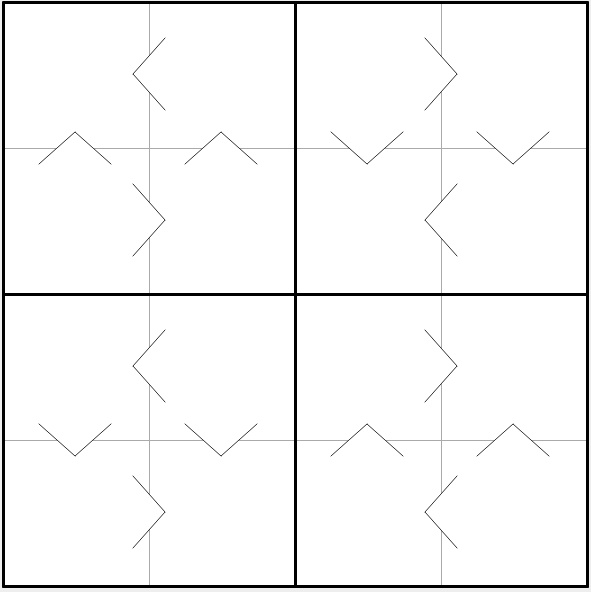
\includegraphics[width=0.4\textwidth]{cs1.jpg}
    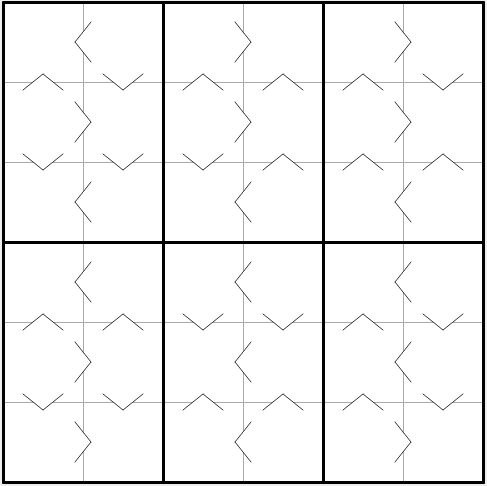
\includegraphics[width=0.4\textwidth]{cs2.jpg}
    \caption{Sodokus comparativos em ambos os possíveis tamanhos.}
    \label{fig:puzzle}
\end{figure}

\newpage
\section{Solução escolhida}

O método utilizado foi o do \textit{backtracking}, as regras de relação de ordem e de validação foram feitas seguindo as regras originais do Sudoku comparativo. Após a definição das regras o compilador testa as possibilidades, se a validação falhar outras possibilidades são testadas. Como será expandido na conclusão, devido ao alto número de possibilidades tabuleiros maiores que 4x4 possuem complexidade muita alta para serem completados em tempo útil.

\subsection{Entrada de Dados}

Após a definição das células as regras criadas anteriormente de ordenação são utilizadas segundo o problema que foi escolhido no site. Após a definição das regras e do backtracking utilizado pelo Prolog a função validate é chamada recursivamente membro a membro para verificar se o elemento não está repetido, nesta etapa são verificados os membros por linha, bloco e coluna.

Abaixo, segue o código de como seria representado o problema Nº1 do site do Sodoku Comparativo:
\\
\\
\texttt{\% problema4x4 Nr. 1\\
    \% LINHA1\\
    menorQue(A1,A2),\\
    menorQue(A3,A4),\\
    \% LINHA2\\
    menorQue(B1,B2),\\
    maiorQue(B3,B4),\\
    \% LINHA3\\
    maiorQue(C1,C2),\\
    menorQue(C3,C4),\\
    \% LINHA4\\\
    maiorQue(D1,D2),\\
    maiorQue(D3,D4),\\
    \% COLUNA1\\\
    maiorQue(A1,B1),\\
    maiorQue(C1,D1),\\
    \% COLUNA2\\\
    menorQue(A2,B2),\\
    menorQue(C2,D2),\\
    \% COLUNA3\\\
    menorQue(A3,B3),\\
    menorQue(C3,D3),\\
    \% COLUNA4\\\
    maiorQue(A4,B4),\\
    maiorQue(C4,D4),\\
}

A versão 6x6 da entrada de dados conta com funções específicas para suprir as necessidades de representar mais combinações, com regras como por exemplo a \texttt{menorMenorMenor}.

Abaixo encontra-se um trecho de definições das regras do exercício Nº4 utilizando as regras mencionadas anteriormente.

\texttt{
\\
\% problema 6X6 Nr. 4\\
\% LINHA1\\
menorMaiorMaior(A1, A2, A3, A4, A5, A6),\\
\% LINHA2\\
maiorMaiorMaior(B1, B2, B3, B4, B5, B6),\\
\% LINHA3\\
menorMenorMenor(C1, C2, C3, C4, C5, C6),\\
}

\subsection{Processamento de Dados}

A computação da solução é realizada na regra \texttt{solve(Solution)}, que pode ser chamada utilizando o Swipl para obter uma solução para o problema dado.
A solução começa com a criação da matriz Solution:
\\
\\
6x6:

\texttt{Solution = [
    	[A1, A2, A3, A4, A5, A6],
    	[B1, B2, B3, B4, B5, B6],
    	[C1, C2, C3, C4, C5, C6],
    	[D1, D2, D3, D4, D5, D6],
    	[E1, E2, E3, E4, E5, E6],
    	[F1, F2, F3, F4, F5, F6]
	]}
\\
\\
4x4:

\texttt{ Solution = [
        [A1, A2, A3, A4],
        [B1, B2, B3, B4],
        [C1, C2, C3, C4],
        [D1, D2, D3, D4]
    ]}
\\
\\
Depois é realizada a entrada de dados do programa, como explicado na seção anterior. Basta então realizar a chamada recursiva para testar valores de acordo com as condições propostas:
\\
\\
4x4:
\\
\texttt{validate([A1, A2, A3, A4]),\\
      validate([B1, B2, B3, B4]),\\
      validate([C1, C2, C3, C4]),\\
      validate([D1, D2, D3, D4]),\\
      validate([A1, A2, B1, B2]),\\
      validate([A3, A4, B3, B4]),\\
      validate([C1, C2, D1, D2]),\\
      validate([C3, C4, D3, D4]),\\
      validate([A1, B1, C1, D1]),\\
      validate([A2, B2, C2, D2]),\\
      validate([A3, B3, C3, D3]),\\
      validate([A4, B4, C4, D4]).}
\\
\\
\\
6x6:

\texttt{
    \\
    \%verifica se não há elementos repetidos nas linhas\\
	validate([A1, A2, A3, A4, A5, A6]),\\
	validate([B1, B2, B3, B4, B5, B6]),\\
	validate([C1, C2, C3, C4, C5, C6]),\\
	validate([D1, D2, D3, D4, D5, D6]),\\
	validate([E1, E2, E3, E4, E5, E6]),\\
	validate([F1, F2, F3, F4, F5, F6]),\\
 	\\
	\%verifica se não há elementos repetidos nas grades\\
	validate([A1, A2, B1, B2, C1, C2]),\\
	validate([A3, A4, B3, B4, C3, C4]),\\
	validate([A5, A6, B5, B6, C5, C6]),\\
	validate([D1, D2, E1, E2, F1, F2]),\\
	validate([D3, D4, E3, E4, F3, F4]),\\
	validate([D5, D6, E5, E6, F5, F6]),\\
    \\
	\%verifica se não há elementos repetidos nas colunas\\
	validate([A1, B1, C1, D1, E1, F1]),\\
	validate([A2, B2, C2, D2, E2, F2]),\\
	validate([A3, B3, C3, D3, E3, F3]),\\
	validate([A4, B4, C4, D4, E4, F4]),\\
	validate([A5, B5, C5, D5, E5, F5]),\\
	validate([A6, B6, C6, D6, E6, F6]).\\}
	
A função validate, conforma foi explicado anteriormente, realiza a verificação de que o elemento não está repetido, por linha, bloco e coluna.
\\
\\
\texttt{validate([]) :- !.\\
	validate([H|T]) :- not(member(H,T)), validate(T).}

\section{Problemas Encontrados}

Para facilitar a implementação, separamos dois resolvedores, um para o puzzle de tamanho 4x4 e outro para o puzzle de tamanho 6x6 ao invés de gerar uma solução genérica, o que tomaria mais tempo.

No puzzle 6x6 o problema se torna maior, temos mais possibilidades e o backtracking não se torna a melhor estratégia de solução. O código deste trabalho leva alguns minutos para resolver o exercício Nº1 tamanho 4x4 e o exercício Nº4 tamanho 6x6.

\end{document}
